\RequirePackage{fix-cm}
\documentclass[12pt,titlepage,openany]{book}

\usepackage{fixltx2e}
\usepackage[xetex]{graphicx}
\usepackage[nottoc,section]{tocbibind}
\usepackage[xetex,bookmarks]{hyperref}
\usepackage{bookmark}
\usepackage{xltxtra}
\usepackage[paper=letterpaper, margin=1in]{geometry}
\usepackage{layout}
\usepackage{multicol}
\usepackage{wrapfig}
\usepackage{calc}
\usepackage{etoolbox}
\usepackage{ccicons}
\usepackage[shortcuts]{extdash}
\usepackage{titling}
\usepackage[nodayofweek,24hr]{datetime}
\usepackage[monochrome,table]{xcolor}
\usepackage{environ}
\usepackage{longtable}
\usepackage{epsfig}
\usepackage[sectionbib,sort,numbers]{natbib}
\usepackage[shortlabels]{enumitem}
\usepackage{float}
\usepackage{lettrine}
\usepackage{titlesec}
\usepackage[strict]{changepage}
\usepackage{lipsum}

\newfontfamily\startrek{Star Trek Enterprise Future}
\newfontfamily\fatefont{Fate Core Glyphs}
\newfontfamily\handwritingfont[Scale=0.9]{Permanent Marker}

\setmainfont[Ligatures={Common,TeX}, Numbers={Proportional}]{Linux Libertine O}
\setmonofont[Scale=0.9]{Luxi Mono}

\urlstyle{same}

\titleformat{\chapter}[display]%
    {\fontsize{0.65in}{0.4in}\selectfont\startrek}%
    {\chaptertitlename~\thechapter}%
    {15pt}%
    {\fontsize{0.75in}{0.4in}\selectfont\startrek}

\titleformat{\section}[hang]%
    {\fontsize{0.4in}{0.3in}\selectfont\startrek}%
    {\thesection}%
    {20pt}%
    {\fontsize{0.4in}{0.3in}\selectfont\startrek}

\titleformat{\subsection}[hang]%
    {\fontsize{0.3in}{0.2in}\selectfont\startrek}%
    {\thesubsection}%
    {15pt}%
    {\fontsize{0.3in}{0.2in}\selectfont\startrek}

\titlespacing*{\section}{0pt}{*6}{*2}
\titlespacing*{\subsection}{0pt}{*4}{*1}

\renewcommand{\dateseparator}{.}

\newdateformat{mydate}{%
    \ifshowdow\dayofweekname{\THEDAY}{\THEMONTH}{\THEYEAR}\fi
    \THEDAY{} \monthname[\THEMONTH{}] \THEYEAR{}%
}

\makeatletter
\long\def\@makefntext#1{%
    \parindent 1em\noindent\hb@xt@ 1.8em{\hss\@makefnmark}~#1%
}
\makeatother

\newenvironment{example}[0]{%
    \begin{quotation}\noindent\itshape\textbf{Example:}%
}{%
    \end{quotation}%
}

\NewEnviron{NewSkillAction}[2][]{%
    \begin{adjustwidth}{40pt}{}%
       \makebox[0pt][r]{\raisebox{-10pt}[0pt][0pt]{%
           \fontsize{25pt}{0pt}\selectfont\SkillActionIcon{#2}%
           \hspace{5pt}%
       }}%
       \textbf{\SkillActionName{#2}:} \BODY%
    \end{adjustwidth}%
    \ifstrequal{#1}{+}{\vspace{\baselineskip}}{}%
    \vspace{1ex}%
}

\newlength{\currentparindent}
\NewEnviron{SkillActionList}{%
    \setlength{\currentparindent}{\parindent}%
    \begin{longtable}[l]{p{25pt}p{\linewidth-45pt}}%
        \BODY%
    \end{longtable}%
    \vspace{-1.5em}%
}

\newcommand{\SkillActionEntry}[2]{%
    \raisebox{-11pt}{\Huge\SkillActionIcon{#1}}&%
    \setlength{\parindent}{\currentparindent}%
    \noindent\textbf{{\SkillActionName{#1}:}} #2 \\ & \\%
}

\newcommand{\skillitem}[1]{%
    \item[{\raisebox{-10pt}[0pt][0pt]{\Huge\fatefont{}{#1}\vspace{10pt}}}]%
}

%\newlength{\currentparindent}
\NewEnviron{SkillAction}[1]{%
    \noindent%
    \setlength{\currentparindent}{\parindent}%
    \parbox[t]{7ex}{\vskip0pt\Huge\fatefont {#1}}%
    \hfill%
    \parbox[t]{\linewidth-7ex}{%
        \vskip0pt%
        \setlength{\parindent}{\currentparindent}%
        \noindent\textbf{{\SkillActionName{#1}}:}
        \BODY%
    }%
}

\newlength{\SkillBoxWidth}
\setlength{\SkillBoxWidth}{6.2em}
\newcommand{\SkillBox}[1]{%
\framebox{\parbox[c][1em][c]{\SkillBoxWidth}{\centering\upshape\handwritingfont #1}}%
    \hspace{3pt}%
}

\newcommand{\blankpage}{%
    \newpage%
    \thispagestyle{empty}%
    \mbox{}%
    \newpage%
}



\geometry{bindingoffset=0in}

\title{Star Trek: Fate}
\author{Chris Bouchard}
\date{\yyyymmdddate\today}

\pagenumbering{gobble}

\begin{document}

\begin{titlepage}
    \pdfbookmark{STAR TREK: Powered by FATE}{Title Page}
    \vspace*{0.5in}
    \begin{center}
        
\includegraphics[height=2.5in]{img/CommBadge.eps}\\
        \vspace*{0.4in}
        {\fontsize{0.75in}{1em}\selectfont\STFLogo}\\
        \vspace*{\fill}
        {\fontsize{0.3in}{1em}\selectfont{}\theauthor}\\
        \vspace*{0.2in}
        {\fontsize{0.25in}{1em}\selectfont{}\thedate}
    \end{center}
\end{titlepage}

\cleardoublepage

\begin{center}
    \parbox{0.85\linewidth}{\begin{center}
    \small\setlength{\parskip}{\baselineskip}
    Star Trek: Fate\\
    Copyright \copyright\ 2013--\the\year\ Chris Bouchard

    {\Huge\ccbync}

    This work is licensed under a Creative Commons Attribution\-/NonCommercial
    license. To view a copy of this license, visit
    \url{http://creativecommons.org/licenses/by-nc/4.0/}.

    First published in 2013 by Chris Bouchard.

    Fate\texttrademark\ is a trademark of Evil Hat Productions, LLC. The
    Powered by Fate logo is \copyright\ Evil Hat Productions, LLC and is used
    with permission.

    This work is based on Fate Core System and Fate Accelerated Edition (found
    at \url{http://www.faterpg.com/}), products of Evil Hat Productions, LLC,
    developed, authored, and edited by Leonard Balsera, Brian Engard, Jeremy
    Keller, Ryan Macklin, Mike Olson, Clark Valentine, Amanda Valentine, Fred
    Hicks, and Rob Donoghue, and licensed for our use under the Creative
    Commons Attribution 3.0 Unported license
    (\url{http://creativecommons.org/licenses/by/3.0/}).

    This work is also based on the Fate System Toolkit (found at
    \url{http://www.faterpg.com/}), a product of Evil Hat Productions, LLC,
    developed, authored, and edited by Robert Donoghue, Brian Engard, Brennan
    Taylor, Mike Olson, Mark Diaz Truman, Fred Hicks, and Matthew Gandy, and
    licensed for our use under the Creative Commons Attribution 3.0 Unported
    license.

    Star Trek, Star Trek: The Animated Series, Star Trek: The Next Generation,
    Star Trek: Deep Space Nine, Star Trek: Voyager, and Star Trek: Enterprise
    are all registered trademarks of CBS Corporation. We offer no suggestion
    that this work is ``official'' or produced or sanctioned by the owner of
    the aforementioned trademarks. We make no claim to own Star Trek or any of
    the names related to it.

    This work is based on material found on Memory Alpha (found at
    \url{http://en.memory-alpha.org/}) and licensed for our use under the
    Creative Commons Attribution\-/NonCommercial 2.5 Generic license
    (\url{http://creativecommons.org/licenses/by-nc/2.5/}).
\end{center}

}
\end{center}
\cleardoublepage

\tableofcontents
\cleardoublepage

\pagenumbering{arabic}



\chapter{Introduction}\label{chap:intro}

\begin{center}
\textit{``Space: The final frontier. These are the voyages of the starship\ldots''}
\end{center}

\vspace{1em}

\noindent
\lettrine[lines=1]{W}{elcome} to \StarTrekFate{}, an adaptation of the
\FateCore{} system for the \StarTrek{} universe.

\section{What You Need to Play}

We assume that you have access to the \FateCore{} book, EHP0001 \textit{Fate
Core System}. This document simply describes the new rules and rules changes we
have made and clarifies some interactions. We will refer to page numbers in the
2013 hard-cover printing.

In addition to the materials described in the section What You Need to Play on
page 3 of the \FateCore{} book, we also recommend that you have access to
``official Federation records'' --- some reference for the \StarTrek{} setting
that your entire group agrees to follow. This document was created using Memory
Alpha,\footnote{Memory Alpha: \url{http://www.memory-alpha.org}} a public
\StarTrek{} wiki.

\section{Play Style}

The \FateCore{} system is designed for collaborative storytelling, and we
strongly encourage that in \StarTrekFate{}. We have not worked out rules
systems for every creature or piece of tech in Federation space. Rather, we
expect that players and GMs will work together to do what seems right. This
only works if players are ``good'' roleplayers, by which we mean focused on
characters and plot rather than stats and rules. The rules are certainly
important (which is why this document exists), but after all the fun of
\StarTrek{} is exploring the unknown!



\chapter{\StarTrek{} Life}\label{chap:life}

\begin{figure}[H]
    \centering
    
\includegraphics[width=0.5\linewidth]{img/Federation.eps}
\end{figure}

\section{Living in the Federation}

\begin{center}
\textit{``A dream that became a reality and spread throughout the stars.''\\
--- Captain James T. Kirk, 2269}
\end{center}

\noindent
The assumed setting for \StarTrekFate{} is the United Federation of Planets, or
at least somewhere within the Alpha Quadrant. This is the part of the galaxy
explored in the majority of the \StarTrek{} franchise. Your characters are
likely Federation citizens, and if not they are very familiar with it.

The big thing to remember about the Federation is that it is a utopian society.
It was founded on the principles of universal liberty, rights, and equality. In
this setting, things like poverty, huger, racism, and even currency have been
largely eradicated for hundreds of years.

This is not to say that your character or the society in which he or she lives
is perfect. The Federation is is still made up of people --- Humans, Vulcans,
Tellarites, and a multitude of other species, but still people. Poverty may be
a thing of the past, but politics can be as ugly and underhanded as ever.
Racism among Humans is considered old-fashioned, but the man on the street
probably has a thing or two to say about ``those Klingons''. The point is that
\StarTrek{} is always \emph{hopeful}. Of course things are not perfect, but
they can be fixed.

\section{Starfleet}

The main focus of \StarTrek{} has always been Starfleet, and this game is no
different. Starfleet is the deep-space exploratory and defense service of the
Federation, and it captures all the ideals of Federation society. Starfleet

There are two ways your character could have joined Starfleet: enlisting or
attending Starfleet Academy.

\subsection*{That's an Order!}\label{subsec:orders}

Starfleet officers and personnel give and obey orders on a daily basis. When
one character wishes to give an order to another, there are several ways the GM
can choose to resolve the situation depending on the situation and the
characters involved.

For most orders from a superior to a subordinate, no special action will be
needed. This is Starfleet, and your character is a trained professional.
Unless your character has a good reason, he or she should generally follow the
orders of superior officers without a fight.

Some orders, however, are simply unacceptable. Such orders may conflict with
one of your character's aspects, or they may be a violation of Starfleet
regulations. In this case, the GM has two options for resolution. He or she
may choose to compel your character's rank aspect, in which case refer to the
\nameref{sec:aspects-orders} section of the \nameref{chap:aspects} chapter.
Otherwise, the order can be resolved using social combat --- or even physical
combat if it comes to it. This option should be saved as a last resort, since
it represents true insubordination.

Finally, for characters outside of Starfleet, the orders of an officer do not
have the same impact. In this case, social combat is the only appropriate way
for one character to command another.



\chapter{Aspects}\label{chap:aspects}

\lettrine[lines=1]{T}{he} \FateCore{} system uses aspects to help give
characters individuality and personality. In \StarTrekFate{}, will modify this
system slightly, adding an extra aspect and imposing some requirements. This
will reflect how big of a commitment being in Starfleet is for your character,
and how much it has shaped his or her life. This chapter details these
requirements.

\section{High Concept}\label{sec:high-concept}

Joining Starfleet is a major, life-changing decision. Thus, it should be
reflected in your character's high concept. A chief engineer may have the high
concept \aspect{Starfleet Gearhead}. Of course, if your character is not a
member of Starfleet, this requirement does not apply to you, though some other
organization may fill this role for your character, such as a Vulcan scientist
with the high concept \aspect{Researcher of the Science Academy}.

\section{Species}\label{sec:species}

Your character's species is definitely a defining characteristic. The story of
\StarTrek{} is told from the Humans' perspective, so for better or for worse
that is the ``default'' species. A player may choose another species with GM
approval. For common species, especially species that are members of the
Federation, the GM should generally err on the side of allowing the choice.
Starfleet does not discriminate on the basis of species --- there have been
Klingon and even Ferengi officers. A non-Human character must have an aspect
reflecting his or her species, but it need not be the high concept.

\section{Rank}\label{sec:rank}

A character's position in Starfleet is a defining characteristic --- remember,
your character has devoted his or her life to joining and advancing within Star
Fleet. Your character has an extra aspect representing his or her rank. You may
invoke this aspect to draw on your character's experience and training, as well
as the respect his or her rank commands. Your rank aspect may be compelled to
force your character to act as his or her rank dictates, perhaps to follow
distasteful orders or to uphold the Prime Directive.


Different versions of \StarTrek{} have not consistently used the same ranks.
For this setting, we will be using the following set, listed from lowest rank
to highest:

\begin{multicols}{2}
    \raggedcolumns
    \paragraph{Enlisted Personnel:}
    \begin{itemize}
        \item Crewman (3rd--1st Class)
        \item Petty Officer (3rd--1st Class)
        \item Chief Petty Officer
        \item Senior Chief Petty Officer
        \item Master Chief Petty Officer
    \end{itemize}

    \columnbreak
    \paragraph{Junior Officers:}
    \begin{itemize}
        \item Ensign
        \item Lieutenant Junior Grade
        \item Lieutenant
    \end{itemize}

    \paragraph{Senior Officers:}
    \begin{itemize}
        \item Lieutenant Commander
        \item Commander
        \item Captain
    \end{itemize}
\end{multicols}

\noindent \emph{(Note that higher ranks do exist, but will not be available at
character creation.)}

\vspace{1em}

If your character is not a member of Starfleet, you may use this aspect to
denote your character's rank within some other similar organization, such as a
Romulan with the aspect \aspect{Centurion} or a Vulcan with the aspect
\aspect{High Priest}. If your character is not a member of any such
organization, your character should have the aspect \aspect{Civilian}.

\section{Aspects and Orders}\label{sec:aspects-orders}

Giving and obeying orders is part and parcel of having a rank, and thus it is
core to your Starfleet character. An order starts as two characters talking.
When a captain gives an order to an ensign, for example, this does not
necessarily create a compel. However, if the GM or the ensign's player feel the
order is unreasonable, the GM may choose to compel the ensign's rank aspect,
at which point the captain's and ensign's players and the GM work together to
determine how the compel will be fulfilled.

Note that the superior officer's player is not requesting a compel. It would be
unreasonable to expect a player to spend a fate point for every order his or
her character gives --- commanding officers would quickly lose control of the
ship. However, if the superior officer's player wishes to have control over
how the subordinate's rank aspect is compelled, or to compel a different
aspect, he or she will need to request a compel as usual.

\begin{example}
    Mary's character Captain Jennings orders Dr.\ Smith to wake a captured
    Romulan centurion for questioning. Dr.\ Smith, played by John, knows that
    this would likely kill the centurion. John says Dr.\ Smith would probably
    refuse that order, since it conflicts with his aspect \aspect{Do No Harm}.
    The GM decides to compel Dr.\ Smith's rank aspect \aspect{Commander} to
    obey the order, and suggests as a compromise that Dr.\ Smith could file an
    official complaint in the medical log. John accepts the fate point, and
    after strong protest Dr.\ Smith wakes the Romulan.
\end{example}

A compel on a character's rank aspect can be bought off (just like any other
compel) by spending a fate point. However, a character should have strong
reason for doing so, such as personal bias or finding an order to be downright
unacceptable.



\chapter{Skills}\label{chap:skills}

\lettrine[lines=1]{A}{s} much as possible, skills work the same in
\StarTrekFate{} as they do in \FateCore{}. However, the setting of \StarTrek{}
is different enough that we felt some changes were required. We decided to
change the way skills are chosen at character creation. The skills Provoke and
Rapport have been removed (they are now covered by the new skill Presence).
Also, several skills have been renamed: Crafts to Engineering, Drive to Pilot,
and Lore to Academics. Finally, some new skills have been added: Bureaucracy,
Medicine, Presence, and Survival. This chapter details the changes we made.

Here is the final skill list for this game:

\begin{multicols}{3}
    \raggedcolumns
    \begin{itemize}
        \item Academics
        \item Athletics
        \item Bureaucracy
        \item Burglary
        \item Contacts
        \item Deceive
        \item Empathy
        \item Engineering
        \item Fight
        \item Investigate
        \item Medicine
        \item Notice
        \item Physique
        \item Pilot
        \item Presence
        \item Resources
        \item Shoot
        \item Stealth
        \item Survival
        \item Will
    \end{itemize}
\end{multicols}

\section{Skill Points}\label{sec:skill-points}

For character creation, we have decided to replace the skill pyramid described
in \FateCore{} in favor of a point-based system.\footnote{This system should be
familiar to players who have played the \emph{Dresden Files RPG}.} Characters
start with a pool of skill points and all skills at \AdjLevel{0}. Players
then spend skill points as described in the section Advancement and Change in
the \FateCore{} book. In the end, skills must still be arranged in \emph{skill
columns}, which means you may not have more skills at any given rank than you
have at the rank below.

The number of skill points given to new characters should be determined by the
GM when he or she designs the campaign. The \FateCore{} book recommends 20, but
we feel this may be too few to represent the amount of training Starfleet
officers and personnel have received. Somewhere between 20 and 30 points is
probably appropriate, based on the desired power-level.

You may not choose to bank skill points received during character creation as
you could skill points acquired at milestones. These skill points represent
your character's past experience and training.

\begin{example}
    The GM has allotted each player 25 skill points for character creation.
    John decides he wants to build a doctor. He knows that the Medicine skill
    will be very important and takes that at \AdjLevel{4}. He wants to play a
    doctor more at home in the lab than the field, so he picks Academics as a
    second \AdjWord{4} skill. John now has 17 skill points remaining, and he
    fills in the remaining skills as follows:

    \begin{center}
        \begin{tabular}{rl}
            \AdjLevel{4} & \SkillBox{Academics}\SkillBox{Medicine}\\[5pt]
            \AdjLevel{3} & \SkillBox{Presence}\SkillBox{Will}\\[5pt]
            \AdjLevel{2} & \SkillBox{Empathy}\SkillBox{Investigate}%
                           \SkillBox{Notice}\\[5pt]
            \AdjLevel{1} & \SkillBox{Athletics}\SkillBox{\small Bureaucracy}%
                           \SkillBox{Contacts}\SkillBox{Deceive}\\[5pt]
                         & \SkillBox{Shoot}\\
        \end{tabular}
    \end{center}
\end{example}

\section{Academics (Lore)}\label{sec:academics}

The Academics skill represents your character's ability to know and find
information. Every Starfleet officer has a degree from Starfleet Academy, so
this skill is about more than simply doing well in school. It's about your
characters aptitude for learning and his or her depth of knowledge in esoteric
subjects. Since a great deal of research is done using AI these days, this is
also the skill for programming and using computers.

\subsection*{Academics Stunts}\label{subsec:academics-stunts}

\begin{itemize}
    \item \stunt{Computer Wizard.} +2 to Academics rolls made to manipulate
        computers.
    \item \stunt{Technobabble.} You can use Academics in place of Deceive when
        attempting to confuse someone with technical jargon.
\end{itemize}

\section{Bureaucracy (New Skill)}\label{sec:bureaucracy}

Bureaucracy is used to navigate the confusing world of Star Fleet regulations.
It not only involves knowing the rules, but also who to talk to and how to do
it.

\begin{SkillActionList}
    \SkillActionEntry{O}{Bureaucracy obstacles are about getting something done
    in a complex organization. They are about knowing obscure by-laws or
    regulatory minutiae, as well as the people and committees involved.}

    \SkillActionEntry{C}{A character can create an advantage using Bureaucracy
    by using the rules to his or her advantage. An example could be citing an
    obscure Starfleet bylaw to win an argument.}

    \SkillActionEntry{A}{Bureaucracy is not used as an attack.}

    \SkillActionEntry{D}{You can use Bureaucracy to defend against other
    actions dealing with the same organization. Usually these will be other
    Bureaucracy actions, but also possibly Contacts or Resources actions.}
\end{SkillActionList}

\subsection*{Bureaucracy Stunts}\label{subsec:bureaucracy-stunts}

\begin{itemize}
    \item \stunt{Work the System.} You may use Bureaucracy in place of Contacts
        when dealing with a large bureaucratic organization.
\end{itemize}

\section{Engineering (Crafts)}\label{sec:engineering}

Engineering is your character's ability to design, build, repair, and otherwise
work with technology. Your character does not necessarily know the theory
behind warp drive (that would be Academics), but he or she sure knows how to
fix one that is threatening to breach.

\subsection*{Engineering Stunts}\label{subsec:engineering-stunts}

To be written.

\section{Medicine (New Skill)}\label{sec:medicine}

Medicine in the 23rd and 24th centuries is a lot more complicated than it used
to be. Doctors now need to know how cells work on a sub-molecular level, as
well as how to use all the technology in a modern sickbay --- not to mention
the physiology of dozens of different species.

Characters can use Medicine to heal others using the wide array of technology
available. Things that used to take a long time to heal, such as broken bones,
can now be corrected all but instantly. Conditions that used to be fatal are
now unpleasant complications. This is not to say that characters are immortal,
just that the line between minor and life-threatening injuries has shifted.

The Medicine skill assumes access to a modern sickbay. Working in the field is
more difficult, with distractions abundant and equipment limited. The available
sickbay is rated\footnote{There is no actual system in place for modifying
Medicine actions based on the available sickbay. It is currently left up to GM
discression.} using the adjective ladder, with a starship sickbay being Good.
Unless otherwise noted, it is always assumed that a doctor has basic tools such
as a medical tricorder.

\begin{SkillActionList}
    \SkillActionEntry{O}{Medicine is the skill for recovering from physical
    consequences (such a skill does not explicitly exist in \FateCore{}). See
    Recovering from a Consequence on page 164 of the \FateCore{} book.
    Depending on the nature of the consequence and the available sickbay, the
    GM may decide that the consequence should be downgraded rather than just
    renamed. This is a judgement call. A consequence should never be downgraded
    by more than one step.

    Medicine can also be used to identify diseases and other medical
    conditions. Again, the GM should take into account the available sickbay
    when deciding on the level of opposition.}

    \SkillActionEntry{C}{Use Medicine to practice ``preventative medicine,''
    giving a character an aspect representing some sort of medican protection.
    Before an away mission, a doctor may prepare a hypospray that gives the
    aspect \aspect{Inoculated for Andorian Shingles}, or perhaps
    \aspect{Oxygenated Blood} if a character will have to survive in a
    high-altitude environment.}

    \SkillActionEntry{A}{Medicine is not really used as an attack. The GM may
    wish to use Medicine as an attack skill to fight some sort of sentient
    virus, but that would be rare.}

    \SkillActionEntry{D}{Similarly, Medicine is not used to defend. Medicine is
    either used before the injury would be inflicted or after. It is difficult
    to imagine a doctor operating on a patient \emph{while} an injury is
    sustained.}
\end{SkillActionList}

\subsection*{Medicine Stunts}\label{subsec:medicine-stunts}

\begin{itemize}
    \item \stunt{Infection Specialist.} +2 to overcome actions with Medicine
        when diagnosing or treating an infection.

    \item \stunt{Field Medic.} If the available sickbay is Fair or lower, treat
        it as one step higher when making Medicine rolls.

    \item \stunt{Walking Tricorder.} You can use Medicine in place of Empathy
        or Notice to assess aspects of other characters if the aspect would be
        discovered in a medical examination.
\end{itemize}

\section{Pilot (Drive)}\label{sec:pilot}

Pilot is the skill of maneuvering starships, shuttles, or any other vehicles.
It presumes proficiency with modern astrogation technology and star maps. This
skill subsumes the Drive skill from \FateCore{}.

\begin{SkillActionList}
    \SkillActionEntry{O}{Use the Pilot skill to plot courses, perform
    maneuvers, know the locations of star systems, or anything else related to
    navigating the galaxy or controlling a ship.}

    \SkillActionEntry{C}{Creating an advantage with Pilot involves flying the
    ship in such a way to confuse enemies or gain a tactical advantage. A conn
    officer may use Pilot to place the aspect \aspect{Hidden in a Nebula} on
    the ship to escape detection, or perhaps the aspect \aspect{Attack Pattern
    Delta} when entering a battle.}

    \SkillActionEntry{A}{Pilot, like Drive, is generally not used as an attack
    skill. \FateCore{} suggests that one could use Drive to attack by ramming.
    However, ramming something with a starship is very different from ramming
    something with an automobile and likely should not be handled as a
    conflict, but rather by placing new aspects on the scene.}

    \SkillActionEntry{D}{Evading attacking ships is the most common defensive
    use of Pilot. Like Drive, Pilot can also be used to defend against
    advantages being created by, or overcome actions of, other ships.}
\end{SkillActionList}

\subsection*{Pilot Stunts}\label{subsec:pilot-stunts}

\begin{itemize}
    \item \stunt{Trick Flyer.} When you succeed with style on a defend action
        with Pilot and choose to reduce the result by one to gain a boost, you
        automatically perform a tricky maneuver to outrun or outflank your
        opponent. You gain a full situation aspect with a free invocation
        instead.
\end{itemize}

\section{Presence (Provoke and Rapport)}\label{sec:presence}

The Rapport and Provoke skills from \FateCore{} have been combined into a
single skill called Presence, which represents a character's force of
personality. In our system, Presence is roughly the mental analog of Fight,
while Empathy, used to read other character's thoughts and emotions, is the
mental analog of Notice. Presence is an active skill, used to affect other
characters in some way.

There is still a certain degree of overlap between Empathy and Presence, since
it can be difficult to move people if one cannot read them. Similarly, though,
it is difficult to be an effective fighter if one is blind. There may be times
when both skills are relevant to an action, though the GM may decide that one
would face a higher level of opposition.

\begin{SkillActionList}
    \SkillActionEntry{O}{You can use your Presence to simply make weak-willed
    (or unimportant) people do or think what you want, whether by charm or by
    intimidation. As with Provoke in \FateCore{}, this will require a contest
    against PCs or important NPCs.}

    \SkillActionEntry{C}{To be written.}

    \SkillActionEntry{A}{Presence can be used as an attack in mental combat,
    just like the Provoke skill in \FateCore{}.}

    \SkillActionEntry{D}{Having a powerful Presence does not make others'
    mental attacks hurt any less. Will is the mental defence skill, or possibly
    Empathy.}
\end{SkillActionList}

\subsection*{Presence Stunts}\label{subsec:presence-stunts}

To be written.

\section{Survival (New Skill)}\label{sec:survival}

The Survival skill is about surviving in rugged conditions --- anywhere that an
average person would not be able to live without training. It could be used to
control one's breathing in a low-oxygen environment, set up camp for an away
mission gone wrong, or follow tracks through wilderness.

\begin{SkillActionList}
    \SkillActionEntry{O}{To be written.}

    \SkillActionEntry{C}{To be written.}

    \SkillActionEntry{A}{Survival is not generally used in conflicts.}

    \SkillActionEntry{D}{Survival is not used to defend against actions.
    Survival is about a character versus the environment.}
\end{SkillActionList}

\subsection*{Survival Stunts}\label{subsec:survival-stunts}

To be written.

\section{A Note about Resources}\label{sec:note-resources}

For most Federation citizens, money and wealth are relics of a sad past.
However, not all species are so ``enlightened'', and sometimes it helps to have
the resources on hand to trade with them. If your character has access to
above\-/average wealth, it can be reflected in the Resources skill. However,
any character in Starfleet with a Resources score should have a reason for it
in his or her backstory. Also be aware that Resources is not very helpful
unless you are in a place where money has value.



\chapter{Starships}\label{chap:starships}

\begin{figure}[H]
    \centering
    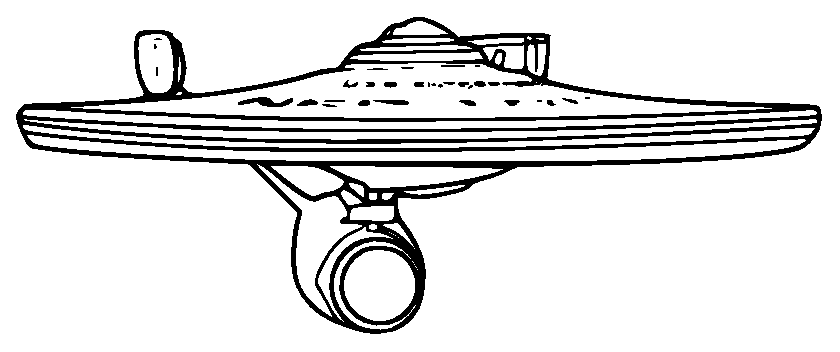
\includegraphics[width=0.8\linewidth]{img/ConstitutionClass.eps}
\end{figure}

\lettrine[lines=1]{A}{ny} captain will tell you that his or her ship is as much
a person as any other member of the crew. Ships seem to have personalities,
temperments, and even character flaws. A Vulcan might say this is simply the
Human tendency to project feelings onto inanimate objects, but that does not
stop the captain from stroking her chair arm to urge the ship on when things
get rough.

\section{Ship Aspects}\label{sec:ship-aspects}

The ship has aspects just like any other character, but there are some
differences. The ship does not have fate points, so its aspects cannot be
\emph{directly} invoked or compelled. Instead, its aspects are treated as
environment aspects when appropriate, and can be invoked by players whose
characters are interacting with the ship. The other difference is that instead
of a rank aspect it has a class aspect, such as \aspect{Constitution-Class}.

Some areas of the ship may have aspects of their own, such as a crew member's
quarters with the aspect \aspect{Meticulously Clean}. Also, areas or the ship
as a whole may gain aspects as a result of combat or plot, like a corridor
gaining the aspect \aspect{Pitch Black} when the power goes out.

\section{Ship Skills}\label{sec:ship-skills}

Just like player characters, not all ships are the same. Some are fast, some
have impressive firepower, and some have cloaking devices. Your ship will have
skills from the following list:

\begin{multicols}{3}
    \raggedcolumns
    \begin{itemize}
        \item Computer
        \item Engine
        \item Maneuver
        \item Security
        \item Sensors
        \item Shields
        \item Stealth
        \item Structure
        \item Weapons
    \end{itemize}
\end{multicols}

The GM will set the number of skill points for the ship at character creation.
Since there are fewer skills for ships, the number should be lower than for
player characters.

There are two ways to assign skills for a ship. The GM may let the players design
the ship from the ground up, including skills. Otherwise, the GM should let the
players pick a ship type, then assign the points him- or herself. In the latter
case, the GM should still keep the players involved as much as possible --- as
always, the goal should be to have fun.

Ship skills are rolled by the GM to see how the ship performs independently of
whoever is controlling it. For example, the ship's sensors only reach so far,
regardless of who is using them. To let a player character control the ship, see
the section on \nameref{sec:control-ship} below.

\section{Ship Stress Tracks and Consequences}\label{sec:ship-stress}

The ship's skills also determine its stress tracks. The ship has two stress
tracks: Shield Strength (determined by the Shields skill) and Structural
Integrity (determined by the Structure skill). Both stress tracks start with
two boxes. If the related skill is \AdjLevel{1} or \AdjLevel{2}, add one box
(for a total of three). If the skill is \AdjLevel{3} or higher, add two boxes
(for a total of four). If the skill is \AdjLevel{5}, the ship also gets an
extra mild consequence.

When the ship takes stress, it is marked on the two stress tracks as follows.
If the shields are active, the stress is marked on the Shield Strength track if
possible. If the shields are active but there is no available box, the shields
buckle and deactivate until they can be repaired. If the shields are inactive,
stress is marked on the Structural Integrity track. If there is no available
box on this track, the ship must either take a consequence or be taken out.

Consequences for the ship reflect big hits that cause lasting damage, and the
crew may get tossed around. When the ship takes a consequence, characters
onboard must defend against a physical attack of a number of shifts equal to
half the shifts of the consequence taken --- 1 shift for a mild consequence, 2
shifts for a moderate consequence, or 3 shifts for a severe consequence.
Athletics or Physique would be appropriate skills to defend against this
attack.

\section{Controlling the Ship}\label{sec:control-ship}

While the ship is sometimes treated as a character, it is still controlled by
its crew. Players may take actions that control the ship, such as a conn
officer changing course or an engineer repairing the warp engines. When
controlling the ship, a player rolls his or her character's relevant skill as
normal, but the result affects the ship rather than the character. In addition,
when controlling the ship, the player can invoke aspects of the ship as well as
those of his or her character.



\chapter{Technology}\label{chap:technology}

\begin{figure}[H]
    \centering
    \raisebox{1.5em}{
\includegraphics[height=1.5in,width=1.5in,keepaspectratio]{img/Phaser2.eps}}
    \hspace*{1em}
    \raisebox{0em}{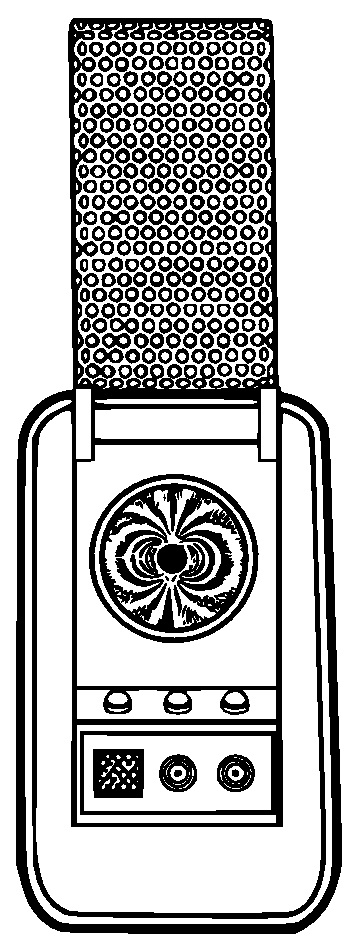
\includegraphics[height=1.5in,width=1.5in,keepaspectratio]{img/Communicator.eps}}
    \hspace*{1em}
    \raisebox{1em}{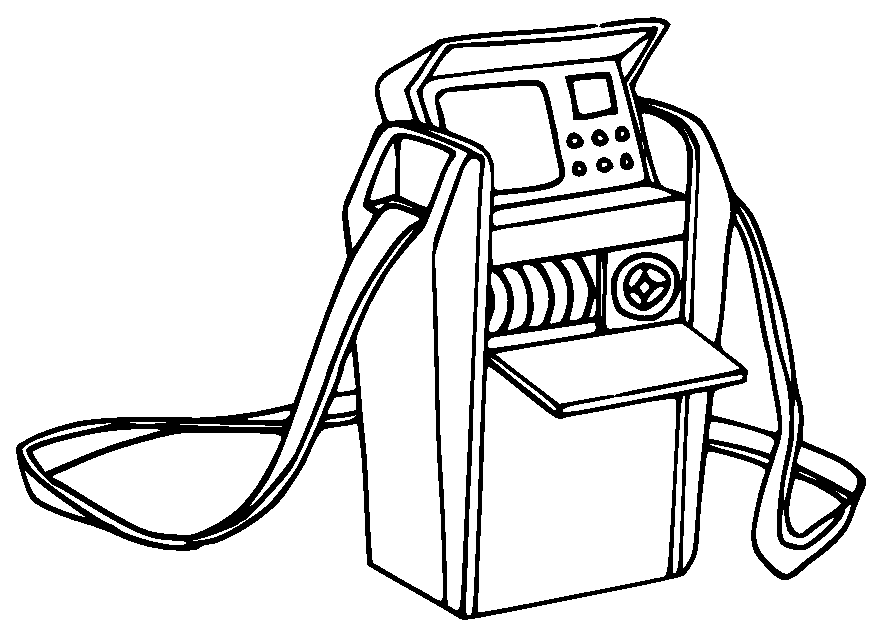
\includegraphics[height=1.5in,width=1.5in,keepaspectratio]{img/Tricorder.eps}}
\end{figure}

\lettrine[lines=1]{T}{here} is an abundance of technology in the \StarTrek{}
universe. Every citizen of the Federation has access to ``basic'' technology
like replicators and subspace communicators. Starfleet makes sure its personnel
are equipped with the latest and greatest.

As much as possible, \StarTrekFate{} tries not to introduce rules for different
pieces of technology --- not only would this be a futile effort, it would be
completely opposed to the \Fate{} philosophy. Characters are assumed to have
whetever equipment is required to perform their jobs.

\begin{wrapfigure}{r}{0.3\linewidth}
    \centering
    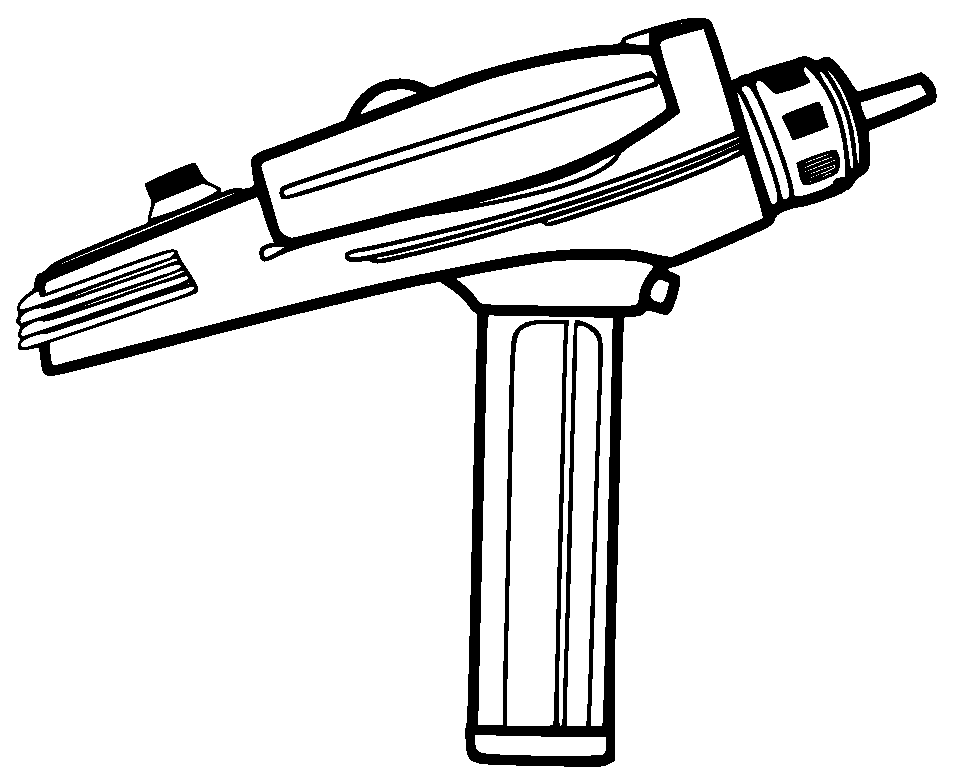
\includegraphics[width=0.8\linewidth]{img/Phaser.eps}\\
    \vspace{2ex}
    \footnotesize A type-2 hand phaser, ca.\ 2260
\end{wrapfigure}

\section{Phasers}\label{sec:phasers}

The standard directed energy weapon of the 23rd and 24th centuries is the
phaser. A phaser fires a nadion particle beam and is as useful a tool as it is
a weapon. Phasers come in a wide variety of shapes and sizes, from small,
handheld devices to massive cannons mounted on starships. Every Starfleet
officer is issued a phaser pistol as their sidearm, and no one graduates the
academy without extensive training in its use and maintenence.

Firing a phaser (unsurprisingly) uses the \skill{Shoot} skill. Phasers have a
multitude of settings, variously described by levels or fractions. Settings are
not described consistently in the various \StarTrek{} shows, so use whatever
description feels right --- as far as this game is concerned, the two modes are
\emph{stun} and \emph{kill}. In stun mode, a character may defend with either
\skill{Athletics} (by dodging and diving) or \skill{Will} (resisting the
stunning effect by force of will). In kill mode, only \skill{Athletics} can be
used to defend. A phaser's setting should be reflected in the types of
consequences taken and the conditions for being taken out by a hit.



\chapter{Species}\label{chap:species}

\end{document}

